% E10 means and sample standard deviations; successful runs only.
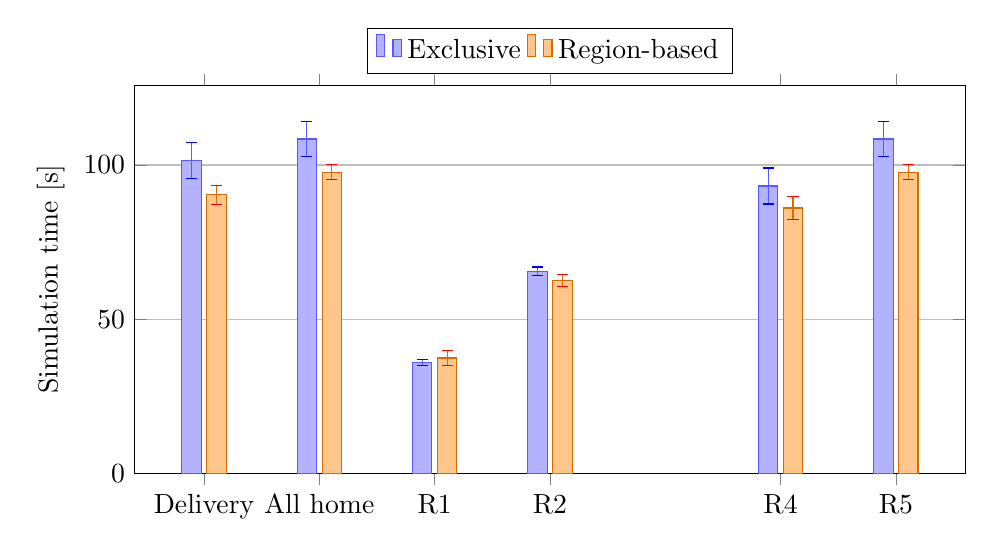
\begin{tikzpicture}
\begin{axis}[ybar,bar width=7pt,width=\linewidth,height=6.5cm,
symbolic x coords={Delivery,All home,R1,R2,R3,R4,R5},xtick=data,ymin=0,ylabel={Simulation time [s]},
legend style={at={(0.5,1.03)},anchor=south,legend columns=2},enlarge x limits=0.1,ymajorgrids=true]
\addplot+[draw=blue!65,fill=blue!30,error bars/.cd,y dir=both,y explicit] coordinates {(Delivery,101.4556) +- (0,5.8069) (All home,108.4444) +- (0,5.8040) (R1,35.8444) +- (0,0.9564) (R2,65.4833) +- (0,1.4420) (R4,93.1944) +- (0,5.8248) (R5,108.4444) +- (0,5.8040)};
\addlegendentry{Exclusive}
\addplot+[draw=orange!85!black,fill=orange!45,error bars/.cd,y dir=both,y explicit] coordinates {(Delivery,90.3722) +- (0,3.0656) (All home,97.6833) +- (0,2.4439) (R1,37.3722) +- (0,2.4223) (R2,62.4556) +- (0,1.9143) (R4,86.0556) +- (0,3.7234) (R5,97.6833) +- (0,2.4439)};
\addlegendentry{Region-based}
\end{axis}
\end{tikzpicture}
